% Results

\begin{slide}{Results}
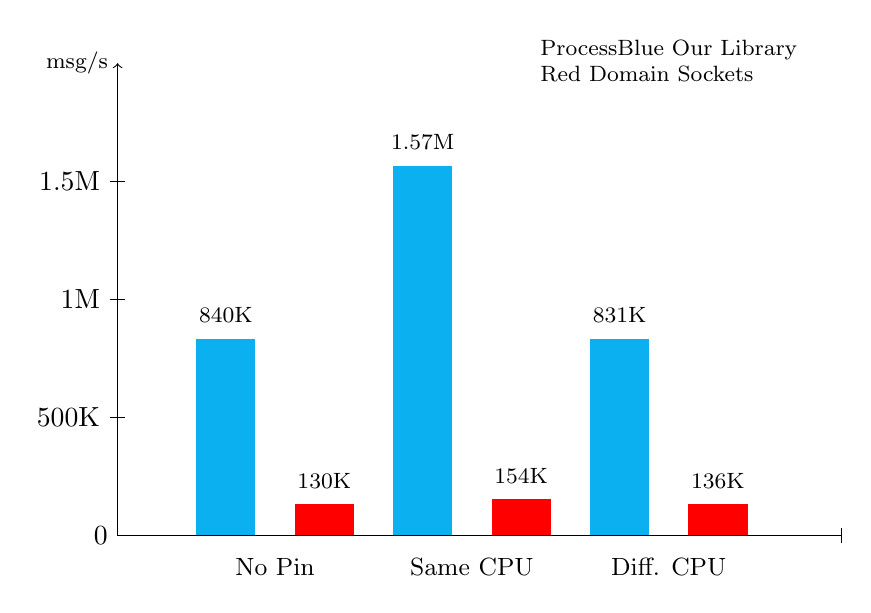
\begin{tikzpicture}

  % No pin
  \onslide<2->{
    % TSSX
    \fill [ProcessBlue] (1, 0) rectangle ++(0.75, 2.5);
    \draw (1.375, 2.8) node {\footnotesize 840K};

    % Domain
    \fill [Red] (2.25, 0) rectangle ++(0.75, 0.4);
    \draw (2.625, 0.7) node {\footnotesize 130K};

    % Label
    \draw (2, -0.4) node {\small No Pin};
  }

  % Different socket
  \onslide<3->{
    % TSSX
    \fill [ProcessBlue] (6, 0) rectangle ++(0.75, 2.5);
    \draw (6.375, 2.8) node {\footnotesize 831K};

    % Domain
    \fill [Red] (7.25, 0) rectangle ++(0.75, 0.4);
    \draw (7.625, 0.7) node {\footnotesize 136K};

    % Label
    \draw (7, -0.4) node {\small Diff. CPU};
  }

  % Same Socket
  \onslide<4->{
    % TSSX
    \fill [ProcessBlue] (3.5, 0) rectangle ++(0.75, 4.7);
    \draw (3.875, 5) node {\footnotesize 1.57M};

    % Domain
    \fill [Red] (4.75, 0) rectangle ++(0.75, 0.46);
    \draw (5.125, 0.76) node {\footnotesize 154K};

    % Label
    \draw (4.5, -0.4) node {\small Same CPU};
  }

  % Legend
  \onslide<2->{
    \draw (7, 6) node {
      \footnotesize
      \begin{tabular}{l}
        \legendsquare{ProcessBlue} Our Library\\
        \legendsquare{Red} Domain Sockets
      \end{tabular}
    };
  }

  % Axes (draw here to overdraw bar borders)
  \draw [-|] (0, 0) node [left] {0} -- (9.2, 0);
  \draw [->] (0, 0) -- (0, 6) node [left] {\footnotesize msg/s};

  \foreach \y/\l in {1.5/500K, 3/1M, 4.5/1.5M} {
    \draw (-0.1, \y) node [left] {\l} -- ++(0.2, 0);
  }
\end{tikzpicture}
\end{slide}

\begin{slide}{Where does this leave us?}
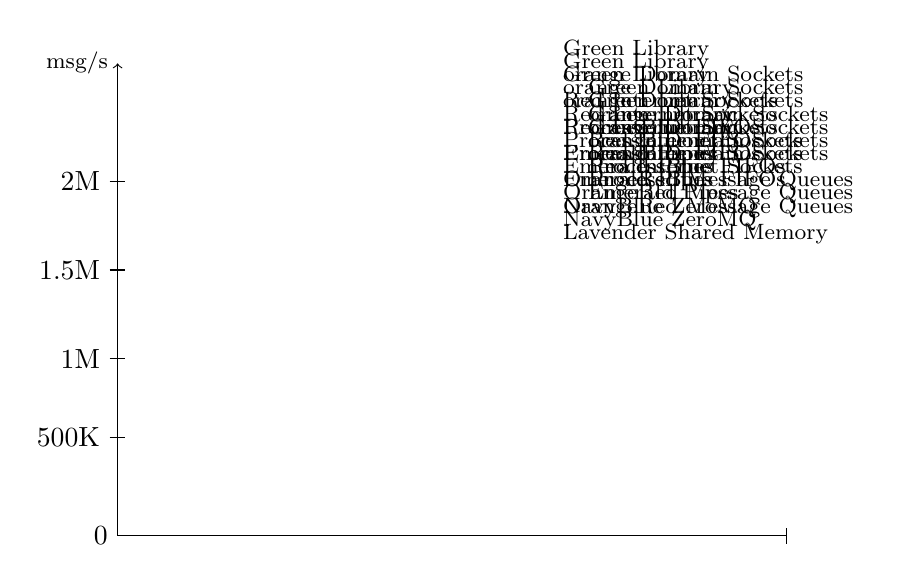
\begin{tikzpicture}
  % TSSX
  \barchart{3.25}{0.75}{3.53}{Green}{1.57M};

  % Domain Sockets
  \barchart{4.25}{0.75}{0.35}{orange}{154K};

  % Internet Sockets
  \onslide<2->{
    \barchart{0.25}{0.75}{0.15}{Red}{67K};
  }

  % FIFOs
  \onslide<3->{
    \barchart{1.25}{0.75}{0.27}{ProcessBlue}{120K};
  }

  % Pipes
  \onslide<4->{
    \barchart{7.25}{0.75}{0.23}{teal}{103K};
  }

  % Message Queues
  \onslide<5->{
    \barchart{5.25}{0.75}{0.4}{OrangeRed}{178K};
  }

  % ZeroMQ
  \onslide<6->{
    \barchart{6.25}{0.75}{0.03}{NavyBlue}{15K};
  }

  % Shared Memory
  \onslide<7->{
    \barchart{2.25}{0.75}{4.95}{Lavender}{2.2M};
  }

  % Legend
  \onslide<1>{
    \draw (7.5, 5) node {
      \footnotesize
      \begin{tabular}{l}
        \legendsquare{Green} Library\\
        \legendsquare{orange} Domain Sockets
      \end{tabular}
    };
  }
  \onslide<2>{
    \draw (7.5, 5) node {
      \footnotesize
      \begin{tabular}{l}
        \legendsquare{Green} Library\\
        \legendsquare{orange} Domain Sockets\\
        \legendsquare{Red} Internet Sockets\\
      \end{tabular}
    };
  }
  \onslide<3>{
    \draw (7.5, 5) node {
      \footnotesize
      \begin{tabular}{l}
        \legendsquare{Green} Library\\
        \legendsquare{orange} Domain Sockets\\
        \legendsquare{Red} Internet Sockets\\
        \legendsquare{ProcessBlue} FIFOs\\
      \end{tabular}
    };
  }
  \onslide<4>{
    \draw (7.5, 5) node {
      \footnotesize
      \begin{tabular}{l}
        \legendsquare{Green} Library\\
        \legendsquare{orange} Domain Sockets\\
        \legendsquare{Red} Internet Sockets\\
        \legendsquare{ProcessBlue} FIFOs\\
        \legendsquare{Emerald} Pipes\\
      \end{tabular}
    };
  }
  \onslide<5>{
    \draw (7.5, 5) node {
      \footnotesize
      \begin{tabular}{l}
        \legendsquare{Green} Library\\
        \legendsquare{orange} Domain Sockets\\
        \legendsquare{Red} Internet Sockets\\
        \legendsquare{ProcessBlue} FIFOs\\
        \legendsquare{Emerald} Pipes\\
        \legendsquare{OrangeRed} Message Queues\\
      \end{tabular}
    };
  }
  \onslide<6>{
    \draw (7.5, 5) node {
      \footnotesize
      \begin{tabular}{l}
        \legendsquare{Green} Library\\
        \legendsquare{orange} Domain Sockets\\
        \legendsquare{Red} Internet Sockets\\
        \legendsquare{ProcessBlue} FIFOs\\
        \legendsquare{Emerald} Pipes\\
        \legendsquare{OrangeRed} Message Queues\\
        \legendsquare{NavyBlue} ZeroMQ\\
      \end{tabular}
    };
  }
  \onslide<7>{
    \draw (7.5, 5) node {
      \footnotesize
      \begin{tabular}{l}
        \legendsquare{Green} Library\\
        \legendsquare{orange} Domain Sockets\\
        \legendsquare{Red} Internet Sockets\\
        \legendsquare{ProcessBlue} FIFOs\\
        \legendsquare{Emerald} Pipes\\
        \legendsquare{OrangeRed} Message Queues\\
        \legendsquare{NavyBlue} ZeroMQ\\
        \legendsquare{Lavender} Shared Memory\\
      \end{tabular}
    };
  }

  % Axes (draw here to overdraw bar borders)
  \draw [-|] (0, 0) node [left] {0} -- (8.5, 0);
  \draw [->] (0, 0) -- (0, 6) node [left] {\footnotesize msg/s};

  \foreach \y/\l in {1.25/500K, 2.25/1M, 3.375/1.5M, 4.5/2M} {
    \draw (-0.1, \y) node [left] {\l} -- ++(0.2, 0);
  }
\end{tikzpicture}
\end{slide}

\begin{slide}{TPC-B Benchmarks}
  \begin{tikzpicture}

    % No pin
    \onslide<2->{
      % TSSX
      \barchart{1.5}{1}{2.5}{ProcessBlue}{45K};

      % Domain
      \barchart{2.75}{1}{1.46}{Red}{25.9K};

      % Label
      \draw (2.6, -0.4) node {\small PostGres};
    }

    % Different socket
    \onslide<3->{
      % TSSX
      \barchart{5.5}{1}{3.7}{ProcessBlue}{65.7K};

      % Domain
      \barchart{6.75}{1}{1.86}{Red}{33.2K};

      % Label
      \draw (6.7, -0.4) node {\small HyPer};
    }

    % Legend
    \onslide<2->{
      \draw (7, 5.5) node {
        \footnotesize
        \begin{tabular}{l}
          \legendsquare{ProcessBlue} Our Library\\
          \legendsquare{Red} Domain Sockets
        \end{tabular}
      };
    }

    % Axes (draw here to overdraw bar borders)
    \draw [-|] (0, 0) node [left] {0} -- (9.2, 0);
    \draw [->] (0, 0) -- (0, 6) node [left] {\footnotesize tps};

    \foreach \y/\l in {2.5/40K, 4.5/80K} {
      \draw (-0.1, \y) node [left] {\l} -- ++(0.2, 0);
    }
  \end{tikzpicture}
\end{slide}
